\documentclass[compress, hide notes]{beamer}
\usetheme{Warsaw} % Beamer Theme
\usecolortheme{lily} % Beamer Color Theme
\useoutertheme[subsection=false]{smoothbars} % Beamer Outer Theme
\useinnertheme{rectangles} 

\usepackage[brazil]{babel}
\usepackage[utf8]{inputenc}

\usepackage{mathrsfs}
\usepackage{tikz}
\usepackage{graphicx}
\usepackage{url}
\usepackage{float}
\usepackage[]{subfigure}
\usepackage{graphicx,color}
\usepackage{scalefnt}
\usepackage{ragged2e}
\usepackage{etoolbox}
\usepackage{beamerthemeshadow}
\usepackage{amsmath,amssymb}
\usepackage{pdfpages}
\usepackage{booktabs}
\usepackage{multirow}
\usepackage{color, colortbl}
\usepackage{verbatim}

\definecolor{Gray}{rgb}{255,215,0}

\newcommand{\specialcell}[2][c]{%
	\begin{tabular}[#1]{@{}c@{}}#2\end{tabular}}

\usepackage{hyphenat}
\hyphenation{des-cre-ve pri-ma-li-da-de u-sa-do pro-ba-bi-li-da-de}

\expandafter\def\expandafter\insertshorttitle\expandafter{%
	\insertshorttitle\hfill%
	\insertframenumber\,/\,\inserttotalframenumber}

\newcommand{\aspas}[1]{``#1''}

%=========================== FULL FRAME IMAGE
\newcommand{\fullframepicture}[1]{
	%\mode
	{
		\usebackgroundtemplate{\includegraphics[width=\paperwidth]{#1}}
		\begin{frame}[plain]
		\end{frame}
	}
	\mode{\usebackgroundtemplate{}}
	%\mode*
}

\usepackage{pgf}
\logo{\pgfputat{\pgfxy(-1.6,-0.1)}{\pgfbox[center,base]{
\includegraphics[width=3cm]{img/logo.jpg}}}}

%fonte arial
\renewcommand{\rmdefault}{phv} % Arial
\renewcommand{\sfdefault}{phv} % Arial

\let\olditem=\item% 
\renewcommand{\item}{\olditem \justifying}%

\graphicspath{{img/}}
	
\setbeamertemplate{navigation symbols}{}

\setbeamertemplate{headline}
{%
	\begin{beamercolorbox}{section in head/foot}
		\vskip2pt\insertsectionnavigationhorizontal{\textwidth}{}{}\vskip2pt
	\end{beamercolorbox}
}




\title[Inteligência Artificial]{\textbf{Inteligência Artificial - \newline \textit{Framework} de Resolução do Problemas de Coloração de Grafo}}

\author[\href{http://buscatextual.cnpq.br/buscatextual/visualizacv.do?id=K8160440H2} {Natanael R.}, \href{http://buscatextual.cnpq.br/buscatextual/visualizacv.do?id=K4868032J4} {Rodolfo L. M. G}.]
{\href{http://buscatextual.cnpq.br/buscatextual/visualizacv.do?id=K8160440H2} {Natanael Ramos}\\ \href{http://buscatextual.cnpq.br/buscatextual/visualizacv.do?id=K4868032J4} {Rodolfo Labiapari Mansur Guimarães}}

\institute{Instituto Federal de Educação, Ciência e Tecnologia de Minas Gerais (IFMG)\\Formiga -- MG -- Brazil}

\date{\today}

%\addtobeamertemplate{footline}{\insertframenumber/\inserttotalframenumber} 

\begin{document}
\frame{\titlepage}

\setbeamertemplate{logo}{}

\AtBeginSection[] {
	\begin{frame}<beamer>
		\frametitle{Sumário} %
		\tableofcontents[currentsection, hideallsubsections]  
	\end{frame}
}

% problema
% exemplo
% como resolveu
% experimentacao (ambiente)
% resultado
%
 
 
 %\import{Introducao}
 

\section{Introdução}
	\begin{frame}{}
		\centering
		\Huge \color{blue} \textbf{Introdução}
	\end{frame}

	\subsection{Motivação}	
	
		\begin{frame}{Motivação \cite{Diego}}
			
			\begin{itemize}
				
				\item \textbf{Metaheurísticas:} estratégias gerais alto-nível que guiam a busca por boas soluções através de busca local.
				
				\bigskip
				
				\item Métodos para problemas intratáveis ou difíceis são comuns na natureza e nas áreas de conhecimento.
				
				\bigskip
				
				\item O proposito é criar uma aplicação flexível para a resolução de problemas para facilitar futuros trabalhos a serem realizados.
				
			\end{itemize}
			
		\end{frame}
		
		
		
\section{Problema}
	\begin{frame}{}
		\centering
		\Huge \color{blue} \textbf{Problema da Coloração de Grafos}
	\end{frame}
	
	\subsection{Introdução}

	\begin{frame}{Problema} %Diego
		\begin{itemize}
        	\item Problema:
            
            \begin{itemize}

                \item Dado um grafo $G = (V, E)$, colorir os vértices de $G$ usando a menor quantidade de cores tal que para cada arco $(i, j) \in E$, os nós $i$ e $j$ tenham cores diferentes.

                \bigskip

                \item Uma $k$-coloração particiona $V$ em $k$ diferentes classes de cores, onde cada membro da classe tem a mesma cor.

                \bigskip

                \item O número cromático $\chi(G)$ de $G$ é o menor inteiro $k$ para o qual $G$ é $k$-colorável.

            \end{itemize}
            
            
            \bigskip
            
            
            \item Aplicação  \cite{Ziviani}:
            \begin{itemize}

                \item Escalonamento de variáveis em registradores de um processador.

                \bigskip

                \item Alocação de horários.

                \bigskip

                \item Alocação de cargas incompatíveis.

            \end{itemize}
            
        \end{itemize}
		
	\end{frame}
	
	\begin{frame}{Problema} %Diego
			
		\begin{figure}[!htb]
			\centering
			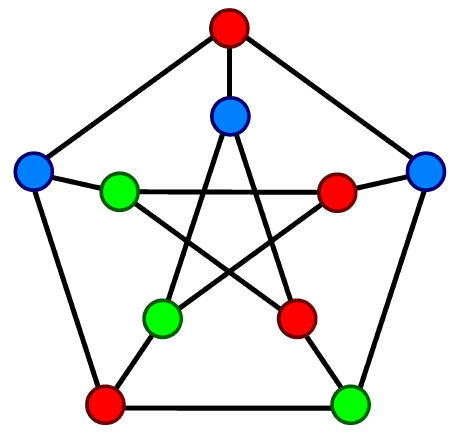
\includegraphics[width=0.6\textwidth]{corExemplo.png}
			\caption{$\chi(G)=3$}
			\label{fig:grafoProblema}
		\end{figure}
		
	\end{frame}


\section{Metodologia}
	\begin{frame}{}
		\centering
		\Huge \color{blue} \textbf{Metodologia de Desenvolvimento}
	\end{frame}

	\begin{frame}{Metodologia}
		
		\begin{itemize}
			
			\item Para solução do problema implementou-se os três métodos, Simulated Annealing, Hill Climbing e Algoritmo Genético.
			
			\bigskip
			
			\item Cada algoritmo possui seu arquivo de configuração.
			
			\bigskip
			
			\item Utilizou-se benchmarks populares desse problema para \\validação da execução.
            
			\bigskip
			
			\item Assim, analisou-se os resultados de cada instância com cada arquivo de configuração.
			
		\end{itemize}
			
	\end{frame}
		
		\subsection{Benchmarks}
		
			\begin{frame}[fragile]{Benchmarks}
				
				\begin{itemize}
					
					\item Foram utilizados para validação e análise dos métodos o conjunto de instâncias \textit{Graph Coloring Instances}\footnote{\url{http://mat.gsia.cmu.edu/COLOR/instances.html}} do Professor da Tepper School of Business da universidade Carnegie Mellon em Pittsburgh, Michael Trick's\footnote{\url{http://mat.gsia.cmu.edu/trick/index.html}}
					
					\bigskip
					
					\item Os arquivos se encontram em formato DIMACS.
					
					\bigskip
					
					\item O \textit{Center for Discrete Mathematics and Theoretical Computer Science} DIMACS\footnote{\url{http://dimacs.rutgers.edu/}} é um centro de pesquisa em matemática discreta, teoria da computação, algoritmos e métodos estatísticos criado em 1989 e sediado em Piscataway - Nova Jersey.
					
					
				\end{itemize}
				
			\end{frame}
			
			\begin{frame}[fragile]{Benchmarks -  Exemplo}
				
					
					{
						\footnotesize
						\begin{block}{}
							
							\begin{verbatim}
							c FILE: anna.col
							c Translated from Stanford GraphBase File: anna.gb
							o 11
							p edge 138 986
							e 1 36
							e 2 45
							e 3 74
							e 4 18
							e 5 36
							e 6 74
							e 6 45
							e 6 136
							e 6 36
							e 6 21
							e 6 18
							e 7 18
							e 7 116
							\end{verbatim}	
						\end{block}
					}
				
			\end{frame}
			
			
			\begin{frame}{Benchmarks}
				
				\footnotesize
				{	
					\begin{table}
						\centering
						\begin{tabular}{l|c|c|c|c|c}
							
							\textbf{Instância}       & \textbf{Vértices} & \textbf{Arestas} & \textbf{Densidade} & \textbf{Ótimo} & \textbf{Fonte}\\ \hline \hline
							mulsol.i.5.col  & 186      & 3973    & 0.231     & 31     &  REG  \\
							queen11\_11.col & 121      & 3960    & 0.545     & 11     &  SGB  \\
							queen13\_13.col & 169      & 6656    & 0.469     & 13     &  SGB  \\
						\end{tabular}
					\end{table}
				}	
                
				\bigskip
				
				\begin{itemize}
					
					\item Os arquivos são divididos por pelo seus criadores e cada um possui uma característica ou origem diferente.
					
					
				\end{itemize}
				
					\scriptsize
					{	
						\begin{table}
							\begin{tabular}{l|c}
								\textbf{Fonte} & \textbf{Descrição}                                                                                                           \\ \hline \hline
								SGB   & \specialcell{Grafos de Donald Knuth em Stanford GraphBase, são baseados em livros,\\ jogos de futebol, cidades dos EUA e Xadrez.} \\\hline
								REG   & Baseado em alocação de variáveis em registradores em códigos reais. \\
							\end{tabular}
						\end{table}
					}
					
			\end{frame}
		
        
        \subsection{Arquivos de Configuração}
        
			
			
			\begin{frame}[fragile]{Arquivo Configuração - Cabeçalho do Arquivo}
				
					
					{
						\footnotesize
						\begin{block}{}
							
							\begin{verbatim}
c Template de arquivo de configuração, 'c' equivale a um comentário

c Método de solução
m <ga|sa|hc>

c Parâmetros dos respectivos métodos 
							\end{verbatim}	
						\end{block}
					}
				
			\end{frame}
			
			\begin{frame}[fragile]{Arquivo Configuração - Simulated Annealing}
				
					
					{
						\footnotesize
						\begin{block}{}
							
							\begin{verbatim}
c Se for o Simulated Annealing

c Quanto menor, mais lento é o decaimento
beta <valor>
c Temperatura inicial
tinit <valor>
c Temperatura final
tfin <valor>
c Número máximo de iterações
samax <valor>
c Quantidade de vizinhos para explorar (Quantity of neighboors)
saqngb <valor>
							\end{verbatim}	
						\end{block}
					}
				
			\end{frame}
			
			\begin{frame}[fragile]{Arquivo Configuração - Hill Climbing}
				
					
					{
						\footnotesize
						\begin{block}{}
							
							\begin{verbatim}
c Se for o Hill Climbing

c Número máximo de iterações
hcmax <valor>
c Quantidade de vizinhos para explorar (Quantity of neighboors)
hcqngb <valor>
							\end{verbatim}	
						\end{block}
					}
				
			\end{frame}
			
			\begin{frame}[fragile]{Arquivo Configuração - Algoritmo Genético}
				
					
					{
						\footnotesize
						\begin{block}{}
							
							\begin{verbatim}
c Se for Genetic Algorithm

c Porcentagem de retorno do Melhor individuo.
taxaMelhorIndividuo <valor>
c Tamanho da populacao em cada iteracao
tamanhoPopulacao <valor>
c Quantidade de gerações de filhos em cada iteração da população
quantidadeGeracoes <valor>
c Porcentagem de aceitação da mutação, ou seja, se o valor
  cfor 0.8, 80% dos inivíduos serão mutados
mutacaoAleatoria <valor>
c Porcentagem para o uso dos métodos de seleção dos pais
  c caso for definido 0.8, 80% será feito com o método do torneio e
  c 20% será realizado com Elite
metodoSelecao <valor>
							\end{verbatim}	
						\end{block}
					}
				
			\end{frame}
        
        
        
        
        
		\subsection{Scripts Extras}
		
			\begin{frame}{Scripts Extras}
				
				\begin{itemize}
					\item Foram utilizados três \textit{scripts} básicos para auxiliar na execução dos métodos e análise estatísticas e visualização de seus resultados, são eles:
					
					%\bigskip
					
					\begin{itemize}
						\item \textit{\textbf{Script Shell:}} utilizado para coordenar de forma autonômica as várias execuções de cada instância do \textit{benchmark} para cada arquivo de configuração.
						
						\bigskip
						
						\item \textit{\textbf{Script R:}} utilizado para leitura seguida de tratamento do arquivo saída das execuções, gerando \textit{boxplots} para análise estatística dos resultados, possibilitando uma comparação entre as duas metaheurísticas.
						
						\bigskip
						
						\item \textit{\textbf{Script DOT:}} utilizado para gerar a representação gráfica do grafo colorido.
					\end{itemize}
					
				\end{itemize}
				
			\end{frame}
            
            
            
		
\section{Implementação Computacional} 

 
 \subsection{Divisão em Módulos}
 
 \begin{frame}{Divisão em Módulos - Objetivo}

     Tentar aproveitar ao máximo o que os métodos tem em comum e separa em \textbf{módulos}:
   %\begin{itemize}
     
   
     \begin{itemize}
     
     	\item Representações: 
        
     	\begin{itemize}
			\item Solução;
            
            \item Grafo;
		\end{itemize}
     
     
     	\bigskip
     
       \item Entrada e saída de dados;
     
     	\bigskip
     
       \item Geração de:
       
       \begin{itemize}
			\item Solução Inicial;
            
            \item Métodos de Pertubação;
		\end{itemize}
       
     
     	\bigskip
     
       \item Configurações e atributos em comum. Exemplo:
     
    	 %\bigskip
     
       \begin{itemize}
         \item Nome dos arquivos de configuração e entrada;
     
         \item Ótimo calculado;
     
         \item Tempo de execução.
       \end{itemize}
     \end{itemize}
  % \end{itemize}
 \end{frame}
 
 
 \subsection{Grafo}
 
 
 
 \begin{frame}{Grafo}
 	
   \begin{itemize}
     \item Uma \textit{hash} de \textit{hash}:
     \bigskip
     \begin{itemize}
     
       \item A primeira mantém um mapeamento de identificadores dos vértices para vizinhos (outra \textit{hash});
     \bigskip
       \item A segunda consiste nos vizinhos de cada vértice, mapeando identificadores e tendo como valor o próprio identificador.
     \end{itemize}
     
     \bigskip     
     
     \item Consistência:
     \begin{itemize}
    	 \item Se um vértice é removido, não precisa-se de tratamento especial para continuar trabalhando na estrutura.
     \end{itemize}
   \end{itemize}
     
 \end{frame}
 
 
 
 \begin{frame}{Grafo}
     
   \begin{itemize}
     \item Eficiência:
     \bigskip
     \begin{itemize}
       \item Busca, inserção e remoção em $O(1)$;
     \bigskip
       \item Verificar se dois vértices são adjacentes: $O(1)$;
     \bigskip
       \item Verificar o grau de um nó: recuperar o tamanho da sua tabela \textit{hash} de vizinhos.
     \end{itemize}
     
     \bigskip
     
     \item Transparência:
     \bigskip
     \begin{itemize}
     	\item O uso da \textit{hash} é encapsulado através de métodos de acesso intuitivos.
     \end{itemize}
   \end{itemize}

 \end{frame}
 
 
 
 \subsection{Representação da Solução}
 
 \begin{frame}{Representação da Solução}
 
   \begin{itemize}
     \item Foram utilizadas duas tabelas \textit{hash}:
     \bigskip
     \begin{itemize}
       \item Uma armazena o mapeamento de vértices para cores atribuídas:
       \begin{itemize}
       	\item Busca, inserção e remoção em $O(1)$.
     \bigskip
     \bigskip
       \end{itemize}
       \item A outra faz o mapeamento do código das cores para sua frequência de utilização:
       \begin{itemize}
         \item Avaliar uma solução: recuperar o tamanho da \textit{hash};
     \bigskip
         \item Busca, inserção e remoção em $O(1)$.
     \bigskip
       \end{itemize}
     \end{itemize}
     \item Relativo baixo consumo de memória, pois armazenam apenas números inteiros.
   \end{itemize}
 
 
 \end{frame}
 
 \subsection{Geração da Solução Inicial}
 
 \begin{frame}
 \frametitle{Geração da Solução Inicial}
 
 \begin{itemize}
 \item A solução inicial pode ser gerada de duas maneiras:
 \bigskip
 \begin{itemize}
 \item Se tem o ótimo calculado:
 \bigskip
 \begin{itemize}
 \item Heurística baseada no teorema das 4 cores de Kempe \cite{kempe1879}.
 \end{itemize}
 \bigskip
 \bigskip
 \item Se não tem:
 \bigskip
 \begin{itemize}
 \item Atribuição aleatória das cores para os nós;
 \end{itemize}
 \end{itemize}
 \end{itemize}
 
 \end{frame}
 
 
 
 \begin{frame}
 \frametitle{Atribuição Aleatória}
 
 \begin{enumerate}
 \item Assume que o máximo de cores $k$ seja igual a quantidade de vértices;
 
 \bigskip
 
 \item Itera os vértices do grafo:
 \begin{enumerate}
 \item Fica em uma laço, sorteando uma dentre as $k$ cores e tentando atribuir ao vértice;
 \begin{itemize}
 \item É necessária a validação com os vizinhos, para não ferir a restrição de que vértices vizinhos tenham a mesma cor.
 
 \bigskip
 
 \end{itemize}
 \item As mesmas cores podem ser sorteadas para vértices diferentes.
 \end{enumerate}
 \end{enumerate}
 
 \end{frame}
 
 
 
 
 \begin{frame}
 \frametitle{Heurística de Kempe}
 
 \begin{enumerate}
 \item Assume que o ótimo encontrado seja $k$;
 
 \bigskip
 
\item Faz uma cópia do grafo original;
 
 \bigskip
 
 \item Itera a cópia do grafo, buscando nós de grau menor ou igual a $k$:
 \begin{enumerate}
 \item Se encontrar, o adiciona a uma pilha e remove da cópia do grafo;
 
 \bigskip
 \bigskip
 
 \item A remoção desses nós leva a reduzir o grau de seus nós vizinhos.
 \end{enumerate}
 
 \bigskip
 
 \item Ao final dessa iteração, começa a atribuir as cores ao vértices da pilha;
 \begin{enumerate}
 \item Fica em uma laço, sorteando uma dentre as $k$ cores e tentando atribuir ao vértice;
 
 \bigskip
 
 \item Ao final, os vértice da pilha são coloridos com no máximo $k$ cores.
 \end{enumerate}
 \end{enumerate}
 
 \end{frame}
 
 \begin{frame}
 \frametitle{Heurística de Kempe}
 \begin{enumerate}
 \setcounter{enumi}{4}
 \item O próximo passo é testar se a cópia do grafo resultante é vazia:
 \begin{enumerate}
 
 \bigskip
 
 \item Se for, então o grafo é $k$-colorível;
 
 \bigskip
 
 \item Caso contrário, precisa de $k+n$ cores:
 
 \bigskip
 
 \begin{enumerate}
 \item Aplica o procedimento de atribuição aleatória ao vértices restantes.
 \end{enumerate}
 \end{enumerate}
 \end{enumerate}
 
 \end{frame}
 
 
 
 
 \subsection{Perturbação da Solução}
 
 \begin{frame}
 \frametitle{Perturbação da Solução}
 
 \begin{enumerate}
 \item Seleciona dois vértice aleatoriamente:
 \begin{itemize}
 \item Que não tenham a mesma cor;
 
 \bigskip
 
 \item Que não sejam o mesmo vértice.
 \end{itemize}
 
 \bigskip
 \bigskip
 
 \item Sorteia uma probabilidade entre $[0,1)$ para escolher uma das cores dos dois vértices;
 \begin{itemize}
 \item Cada um tem a mesma probabilidade de ser escolhido ($50 \%$).
 \end{itemize}
 
 \bigskip
 \bigskip
 
 \item Tenta atribuir essa cor ao outro vértice:
 \begin{enumerate}
 \item Caso consiga, para o algoritmo;
 
 \bigskip
 
 \item Caso não, volta ao passo 1.
 \end{enumerate}
 \end{enumerate}
 
 \end{frame}




 \subsection{Hill Climbing}
 
 			\begin{frame}
				\centering
				{
					\Huge 
					\textcolor{blue}{\textbf{Hill Climbing}}
				}
			\end{frame}
 
 

 \begin{frame}
 \frametitle{Hill Climbing}
 
 \begin{enumerate}
 \item Gera a solução inicial;
 
 
 \bigskip
 \bigskip
 
 \item Fica em um laço de acordo com as iterações máximas especificadas: 
 
 \bigskip
 
 \begin{enumerate}
 \item Gera $n$ vizinhos e verifica:
 \begin{itemize}
 
 \bigskip
 
 \item Caso encontre um vizinho melhor que a solução atual, atualiza e continua o laço;
 
 \bigskip
 
 \item Caso contrário, para o laço e devolve a solução atual.
 \end{itemize}
 \end{enumerate}
 \end{enumerate}
 
 \end{frame}
 
 
 
 
 
 \subsection{Simulated Annealing}
 
 			\begin{frame}
				\centering
				{
					\Huge 
					\textcolor{blue}{\textbf{Simulated Annealing}}
				}
			\end{frame}
 
 \begin{frame}{Simulated Annealing (Adaptado de \cite{Lopes2013})}
 
 \begin{enumerate}
 \item Mantêm três soluções: atual, vizinha e melhor;
 
 \bigskip
 
 \item Gera a solução inicial;
 
 \bigskip
 
 \item Fica em um laço de acordo com a temperatura: 
 \begin{enumerate}
 \item Fica em um segundo laço de acordo com as iterações máximas especificadas:
 \begin{enumerate}
 \item Gera $n$ vizinhos e verifica:
 \item Se a solução vizinha é melhor que a atual, atualiza e verifica se é melhor que a solução estrela (melhor solução).
 \item Caso não seja, sorteia uma probabilidade entre $[0,1)$ e verifica em relação ao critério de aceitação de Boltzmann:
 \item Se a probabilidade for menor que o critério, atualiza a solução atual com a vizinha.
 \end{enumerate}
 
 \bigskip
 
 \item Quando o laço de iterações termina:
 \begin{enumerate}
 \item Reduz a temperatura de acordo com a função de decaimento lento;
 \item Recomeça as iterações.
 \end{enumerate}
 \end{enumerate}
 \end{enumerate}
 
 \end{frame}
 
 

		\subsection{Algoritmo Genético}
			\begin{frame}
				\centering
				{
					\Huge 
					\textcolor{blue}{\textbf{Algoritmo Genético}}
				}
			\end{frame}

			\begin{comment}
            
			\begin{frame}{Estrutura de Dados - Cromossomo}
				\begin{itemize}			
					
					\item O cromossomo é representado pela \textit{Hash}.
					
					\bigskip
					
					\item Cada item é pesquisado utilizando o ID do vértice no qual deseja encontrar sua cor.
					
					\bigskip
					
					\item O valor da cor é representado por números naturais sendo o 0 específico para o estado erro.
					
					\bigskip
					
					\item As cores não são ordenadas/sequências. 
				\end{itemize}
			\end{frame}
            
            \end{comment}
			
			\subsubsection{Estrutura do Algoritmo}
			\begin{frame}{Estrutura Geral do Algoritmo}
				
				\begin{itemize}
					
					\item Algoritmo é executado seguindo as etapas:
					
					\bigskip
					
					\begin{enumerate}
						\item Geração da população inicial;

						\begin{itemize}
							\item Aleatório;
                            \bigskip
							\item Kempe.
						\end{itemize}
						
						\bigskip
						\bigskip
						
						\item Avaliação da população;
						
						\bigskip
						\bigskip
						
						\item Realiza seleção e cruzamento:

						\begin{enumerate}
                        
							\item Seleção dos pais (Elite / Torneio);
							
							\bigskip
							
							\item \textit{Crossover};
							
							\bigskip
							
							\item Mutação.
						\end{enumerate}
						
						\bigskip
						\bigskip
						
						\item Avaliação da população.
					\end{enumerate}
				\end{itemize}
			\end{frame}
			
			\begin{comment}
            
			\subsubsection{Inicializa a População}
			\begin{frame}{Inicializando a População}
				\begin{itemize}

					\item Aleatória (quando não se conheçe o ótimo):

					\begin{itemize}

						\item A população é gerada por indivíduos totalmente aleatórios.
						
						\bigskip
						
						\item Utilizou-se intervalos de $ 1..numVertices $.
						
						\bigskip
						
						\item Serão gerados $ tamPopulacao-1 $ indivíduos. 
						
						\bigskip
						
						\item O último indivíduo gerado para completar a população será feito como sendo o \textbf{pior indivíduo}. Nele cada vértice terá uma cor diferente dos demais.
						
					\end{itemize}


					\bigskip

					\item Kempe (quando se conhece o ótimo);

				\end{itemize}
			\end{frame}
			
			
			\subsubsection{Avalia a população}
			\begin{frame}{Avalia a População}
				\begin{itemize}

					\item É verificado a cor de cada vértice em relação ao seus adjacentes.
					
					\bigskip
					
					\item Se o indivíduo for um grafo colorido válido, seu \textit{fitness} \textbf{recebe a quantidade de cores distintas no cromossomo}. Caso contrário o \textit{fitness} recebe $ 0 $ (zero).
					
					\bigskip
					
					\item Depois da avaliação é realizada uma ordenação da população por meio de seu \textit{fitness}.
					
				\end{itemize}
			\end{frame}
			
			
			
			\subsubsection{Crossover}
			
			\begin{frame}{\textit{Crossover} - Seleção dos Pais \cite{HINDI}}
				\begin{itemize}
					\item Existe dois métodos de seleção de pais:
					
					\bigskip
					
					\begin{itemize}
						\item \textbf{Elite:} São escolhidos \textbf{os dois melhores indivíduos} de toda a população;
						
						\bigskip
						
						\item \textbf{Torneio:} Para a escolha de \textbf{cada pai} são selecionados dois indivíduos aleatoriamente da população. Estes são comparados e será retornado o melhor entre eles. A escolha do melhor ou pior entre eles é feita a partir de uma porcentagem lida do arquivo de configuração.
					\end{itemize}
					
					\bigskip
					
					\item Cada método é escolhido aleatoriamente sendo a probabilidade é descrita no arquivo de configuração.
					
				\end{itemize}
			\end{frame}
			
			
			\begin{frame}{\textit{Crossover} - Recombinação}
				\begin{itemize}
					
					\item A recombinação é feita de forma padrão realizando 1 (um) corte no indivíduo e recombinando os pais gerando 2 novos indivíduos.
					
					\bigskip
					
					\item É escolhido um número aleatório e este é o ponto onde será realizado o corte para a remontagem dos indivíduos.
					
					\bigskip
					
					\item Com este processo, é gerado dois indivíduos.
					
				\end{itemize}
			\end{frame}
			
			
			\begin{frame}{\textit{Crossover} - Mutação  \cite{HINDI}}
				\begin{itemize}
					
					\item A mutação ocorre de maneira simples.
                    \bigskip

					\item Existe uma porcentagem para a execução da mutação.
                    \bigskip

					\item Muta $n$ posições aleatórias sendo $n$ o fator de \\$quantVertices * porceMutacao$ sento o último informado no arquivo de configuração.
					
					
					\bigskip
					\bigskip
					
					\item Depois da mutação, algoritmo não permite adicionar um indivíduo já existente na população.
					
					\bigskip
					
					\item Todos os \textit{dois} indivíduos gerados em cada cruzamento são adicionados na população criando uma super população.
					
				\end{itemize}
			\end{frame}

			\subsubsection{Avalia População e Seleciona o Melhor Indivíduo Já Encontrado}
			\begin{frame}{Avalia População e Seleciona o Melhor Indivíduo Já Encontrado}
				\begin{itemize}
					\item Após gerar todos os indivíduos e formar a super população, realiza-se a avaliação da população.
                    \bigskip

					\item Após a avaliação, realiza-se a ordenação de toda a população.
                    \bigskip

					\item Ordenado, seleciona o melhor indivíduo da super população e compara com o atual.
					
                    \bigskip
                    
					\item Define o melhor entre eles.
				\end{itemize}
			\end{frame}
			
			
			\subsubsection{Seleção Próxima Geração}
			\begin{frame}{Seleção Próxima Geração}
				\begin{itemize}
					\item A população encontra-se com todos os membros antigos e os filhos gerados sobre cada cruzamento.
					
					\bigskip
					
					\item Realiza-se então uma seleção de alguns indivíduos da Elite juntamente com outros não-Elite completando o total da nova população.
                    \bigskip

					\item Optou-se por utilizar uma porcentagem no qual o usuário escolhe a porcentagem de cada classe.
				
					\bigskip
					\bigskip

					\item Todo este processo de Cruzamento e Avaliação da População é realizada $ Geracoes $ vezes.
				\end{itemize}
			\end{frame}

		\end{comment}




	\section{Análise Experimental}
	\begin{frame}{}
		\centering
		\Huge \color{blue} \textbf{Análise Experimental}
	\end{frame}
	
		\subsection{Ambiente de Testes}
		
			\begin{frame}[fragile]{Ambiente de Testes}
				
				\begin{itemize}
					\item Desenvolvimento:
                    
                    \begin{itemize}
						\item Ambos métodos foram implementados em linguagem Java, utilizando a \textit{Integrated Development Environment} IDE Netbeans 8.0.2\footnote{\url{https://netbeans.org/}} e compilador \verb|javac| versão \verb|1.7.0_71| e \verb|1.8.0_45|.
					\end{itemize}
                    
                    \bigskip
                    
                    \item Execução:
                 	
                    
                    \begin{itemize}
						\bigskip
                      \item Dell Inspiron 14R
                      \begin{itemize}
                          \item Processador Intel Core i7-4500U 1.80GHz;
                          \item 7.7 GiB de memória RAM DDR3;
                          \item Sistema Operacional Linux (3.16.0-38-generic) Distribuição Linux Mint 17.2 Rafaela.
                      \end{itemize}


					\end{itemize}
                    
                    
				\end{itemize}
				
			\end{frame}
		
        
        
        
        
		\subsection{Variação de Parâmetros}
		
		
			\subsubsection{Hill Climbing}


				\begin{frame}[fragile]{Variação de Parâmetros - Hill Climbing}
					
					\begin{minipage}{5cm}
						
						\begin{block}{\textbf{hc.config}}
							m hc\\
							hcmax 100\\
							hcqngb 30
						\end{block}
					\end{minipage}\hfill
					\begin{minipage}{5cm}
						\begin{block}{\textbf{hc2.config}}
							m hc\\
							hcmax 500\\
							hcqngb 30
						\end{block}
					\end{minipage}
				\end{frame}
                
                \subsubsection{Simulated Annealing}
				
				\begin{frame}[fragile]{Variação de Parâmetros - Simulated Annealing}
					\begin{minipage}{5cm}
                    
						\begin{block}{\textbf{sa.config}}
							m sa\\
                            beta 0.5\\
                            tinit 100\\
                            tfin 0.1\\
                            samax 100\\
                            saqngb 20
						\end{block}
					\end{minipage}\hfill
					\begin{minipage}{5cm}
                    
						\begin{block}{\textbf{sa2.config}}
                              m sa\\
                              beta 0.5\\
                              tinit 100\\
                              tfin 0.1\\
                              samax 200\\
                              saqngb 20
						\end{block}
					\end{minipage}
				\end{frame}
                
                
                
                \subsubsection{Genetic Algorithm}
				
				\begin{frame}[fragile]{Variação de Parâmetros - Genetic Algorithm}
					\begin{minipage}{5cm}
                    
						\begin{block}{\textbf{ga1.config}}
							m ga\\
                            taxaMelhorIndividuo 0.7\\
                            tamanhoPopulacao 100\\
                            quantidadeGeracoes 50\\
                            mutacaoAleatoria 0.8\\
                            metodoSelecao 0.9\\
                            percMutation 0.2
						\end{block}
					\end{minipage}\hfill
					\begin{minipage}{5cm}
                    
						\begin{block}{\textbf{ga2.config}}
                              m ga\\
                              taxaMelhorIndividuo 0.7\\
                              tamanhoPopulacao 100\\
                              quantidadeGeracoes 50\\
                              mutacaoAleatoria 0.5\\
                              metodoSelecao 0.5\\
                              percMutation 0.2
						\end{block}
					\end{minipage}
				\end{frame}
				
                
                
				\begin{frame}[fragile]{Variação de Parâmetros - Genetic Algorithm}
					\begin{minipage}{5cm}
                    
						\begin{block}{\textbf{ga3.config}}
                              m ga\\
                              taxaMelhorIndividuo 0.7\\
                              tamanhoPopulacao 500\\
                              quantidadeGeracoes 100\\
                              mutacaoAleatoria 0.8\\
                              metodoSelecao 0.9\\
                              percMutation 0.2
						\end{block}
					\end{minipage}\hfill
					\begin{minipage}{5cm}
                    
						\begin{block}{\textbf{ga4.config}}
                              m ga\\
                              taxaMelhorIndividuo 0.7\\
                              tamanhoPopulacao 500\\
                              quantidadeGeracoes 100\\
                              mutacaoAleatoria 0.5\\
                              metodoSelecao 0.5\\
                              percMutation 0.2
						\end{block}
					\end{minipage}
				\end{frame}
                
                
             
	\begin{frame}{}
		\centering
		\Huge \color{blue} \textbf{Função Objetivo}
	\end{frame}   
    
                
	\subsection{Resultados - Função Objetivo}
    
    	\subsubsection{mulsoli5col}
		
        \begin{frame}{Resultados - Hill Climbing (mulsoli5col - opt 31)}
        
        	\begin{figure}[H]
			\centering
            \label{fig:sol-hc-mulsoli5col}
            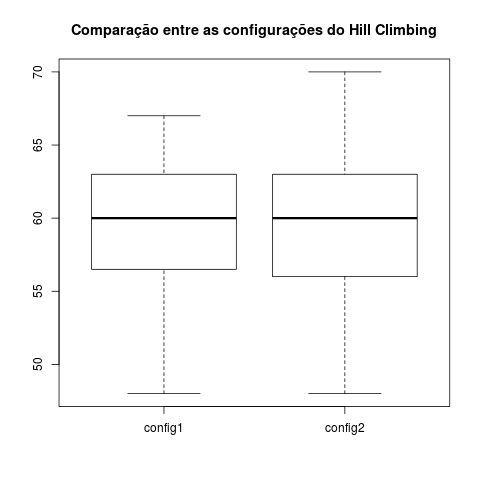
\includegraphics[width=0.6\linewidth]{img/hill-sol-mulsoli5col.png}
            \caption[Resultados para o benchmark mulsoli5col.txt]{Resultados para o benchmark \textit{mulsoli5col.txt}}
			\end{figure}

		\end{frame}
        
        
        \begin{frame}{Resultados - Hill Climbing (mulsoli5col - opt 31)}
        
        	\begin{table}[H]
            \centering
              \begin{tabular}{c|c}
              
               \textbf{config1}       &  \textbf{config2}                        \\ \hline \hline
               Min.   :48.00 &          Min.   :48.00          \\ \hline
               1st Qu.:56.75 &          1st Qu.:56.00          \\ \hline
               Median :60.00 &          Median :60.00          \\ \hline
               Mean   :59.37 &          Mean   :59.65          \\ \hline
               3rd Qu.:63.00 &          3rd Qu.:63.00          \\ \hline
               Max.   :67.00 &          Max.   :70.00          \\ 
              \end{tabular}
              \caption {Dados estatísticos - Hill Climbing}
        	\end{table}

		\end{frame}
        
        
        \begin{frame}{Resultados - Simulated Annealing (mulsoli5col - opt 31)}
        
        	\begin{figure}[H]
			\centering
            \label{fig:sol-sa-mulsoli5col}
            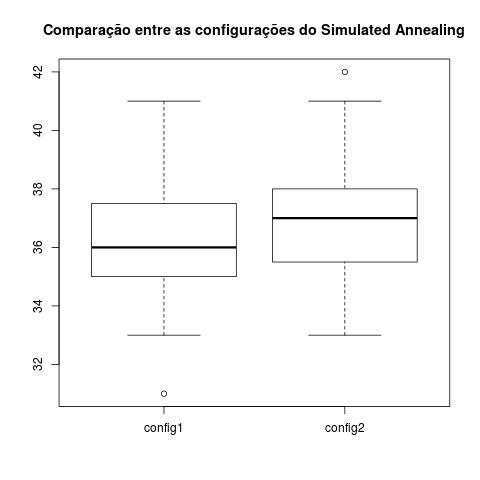
\includegraphics[width=0.5\linewidth]{img/sa-sol-mulsoli5col.png}
            \caption[Resultados para o benchmark mulsoli5col.txt]{Resultados para o benchmark \textit{mulsoli5col.txt}}
			\end{figure}

		\end{frame}
        
        \begin{frame}{Resultados - Simulated Annealing (mulsoli5col - opt 31)}
        
        	\begin{table}[H]
            \centering
              \begin{tabular}{c|c}
               \textbf{config1}       &  \textbf{config2}                        \\ \hline \hline
               Min.   :31.00 &          Min.   :33.00          \\ \hline
               1st Qu.:35.00 &          1st Qu.:35.75          \\ \hline
               Median :36.00 &          Median :37.00          \\ \hline
               Mean   :36.47 &          Mean   :36.69          \\ \hline
               3rd Qu.:37.25 &          3rd Qu.:38.00          \\ \hline
               Max.   :41.00 &         Max.   :42.00           \\ 
              \end{tabular}
              \caption {Dados estatísticos - Simulated Annealing}
        	\end{table}

		\end{frame}
        
        
        
        \begin{frame}{Resultados - Algoritmo Genético (mulsoli5col - opt 31)}
        
        	\begin{figure}[H]
			\centering
            \label{fig:sol-ga-mulsoli5col}
            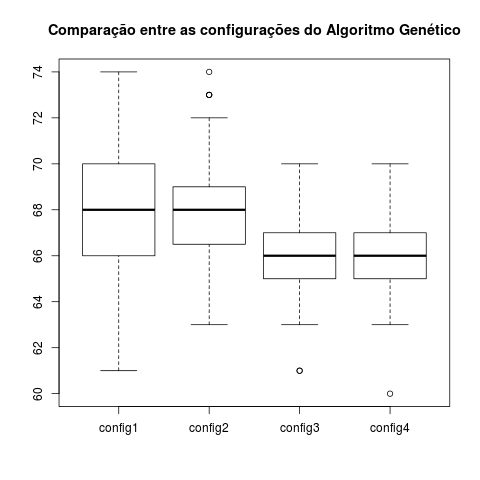
\includegraphics[width=0.6\linewidth]{img/ga-sol-mulsoli5col.png}
            \caption[Resultados para o benchmark mulsoli5col.txt]{Resultados para o benchmark \textit{mulsoli5col.txt}}
			\end{figure}

		\end{frame}
        
        
        \begin{frame}{Resultados - Algoritmo Genético (mulsoli5col - opt 31)}
        
        	\begin{table}[H]
            \centering
              \begin{tabular}{c|c|c|c}
               \textbf{config1}       &  \textbf{config2}               &  \textbf{config3}                &  \textbf{config4}                         \\ \hline \hline
               Min.   :61.00 &          Min.   :63.00 &           Min.   :61.00 &           Min.   :60.00          \\ \hline
               1st Qu.:66.00 &          1st Qu.:66.75 &           1st Qu.:65.00 &           1st Qu.:65.00          \\ \hline
               Median :68.00 &          Median :68.00 &           Median :66.00 &           Median :66.00          \\ \hline
               Mean   :67.91 &          Mean   :68.06 &           Mean   :65.69 &           Mean   :65.88          \\ \hline
               3rd Qu.:70.00 &          3rd Qu.:69.00 &           3rd Qu.:67.00 &           3rd Qu.:67.00          \\ \hline
               Max.   :74.00 &          Max.   :74.00 &          Max.   :70.00  &           Max.   :70.00          \\ 
              \end{tabular}
              \caption {Dados estatísticos - Algoritmo Genético}
        	\end{table}

		\end{frame}
        
        
        
        \subsubsection{queen1111col}
		
        \begin{frame}{Resultados - Hill Climbing (queen1111col - opt 11)}
        
        	\begin{figure}[H]
			\centering
            \label{fig:sol-hc-queen1111col}
            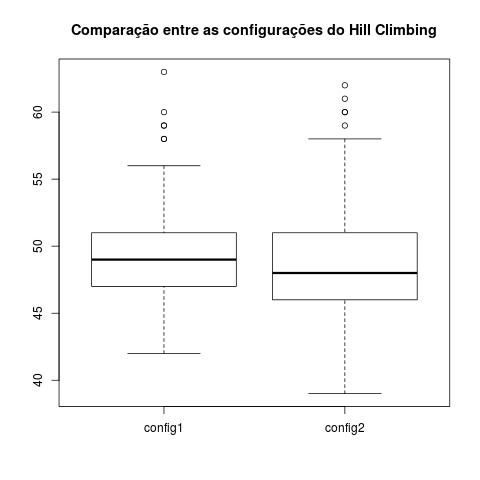
\includegraphics[width=0.6\linewidth]{img/hill-sol-queen1111col.png}
            \caption[Resultados para o benchmark queen1111col.txt]{Resultados para o benchmark \textit{queen1111col.txt}}
			\end{figure}

		\end{frame}
        
        \begin{frame}{Resultados - Hill Climbing (queen1111col - opt 11)}
        
        	\begin{table}[H]
            \centering
              \begin{tabular}{c|c}
               \textbf{config1}       &  \textbf{config2}                        \\ \hline \hline
               Min.   :42.00 &          Min.   :39.00          \\ \hline
               1st Qu.:47.00 &          1st Qu.:46.00          \\ \hline
               Median :49.00 &          Median :48.00          \\ \hline
               Mean   :49.38 &          Mean   :48.82          \\ \hline
               3rd Qu.:51.00 &          3rd Qu.:51.00          \\ \hline
               Max.   :63.00 &         Max.   :62.00           \\ 
              \end{tabular}
              \caption {Dados estatísticos - Hill Climbing}
        	\end{table}

		\end{frame}
        
        \begin{frame}{Resultados - Simulated Annealing (queen1111col - opt 11)}
        
        	\begin{figure}[H]
			\centering
            \label{fig:sol-sa-queen1111col}
            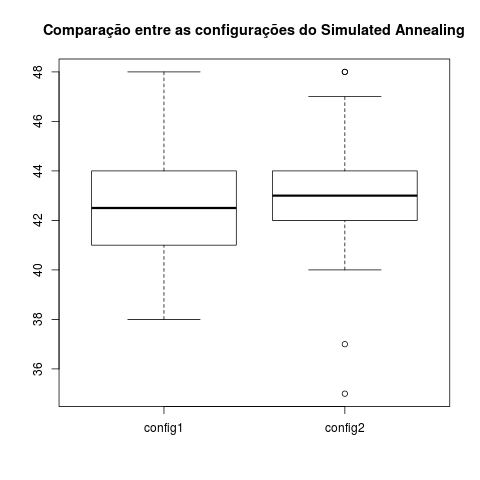
\includegraphics[width=0.6\linewidth]{img/sa-sol-queen1111col.png}
            \caption[Resultados para o benchmark queen1111col.txt]{Resultados para o benchmark \textit{queen1111col.txt}}
			\end{figure}

		\end{frame}
        
        \begin{frame}{Resultados - Simulated Annealing (queen1111col - opt 11)}
        
        	\begin{table}[H]
            \centering
              \begin{tabular}{c|c}
               \textbf{config1}       &  \textbf{config2}                        \\ \hline \hline
               Min.   :38.00 &          Min.   :35.00          \\ \hline
               1st Qu.:41.00 &          1st Qu.:42.00          \\ \hline
               Median :42.50 &          Median :43.00          \\ \hline
               Mean   :42.61 &          Mean   :42.98          \\ \hline
               3rd Qu.:44.00 &          3rd Qu.:44.00          \\ \hline
               Max.   :48.00 &          Max.   :48.00          \\
              \end{tabular}
              \caption {Dados estatísticos - Simulated Annealing}
        	\end{table}


		\end{frame}
        
        \begin{frame}{Resultados - Algoritmo Genético (queen1111col - opt 11)}
        
        	\begin{figure}[H]
			\centering
            \label{fig:sol-ga-queen1111col}
            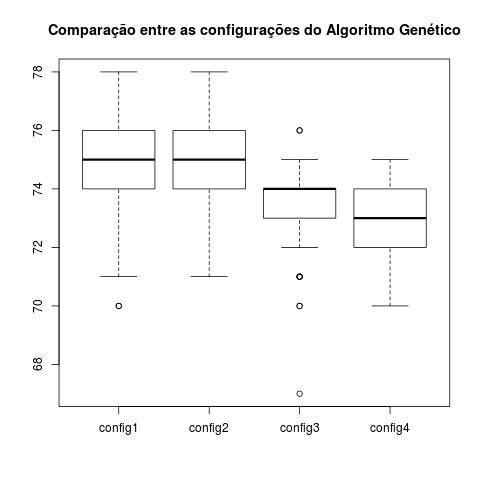
\includegraphics[width=0.5\linewidth]{img/ga-sol-queen1111col.png}
            \caption[Resultados para o benchmark queen1111col.txt]{Resultados para o benchmark \textit{queen1111col.txt}}
			\end{figure}

		\end{frame}
        
        \begin{frame}{Resultados - Algoritmo Genético (queen1111col - opt 11)}
        
        	\begin{table}[H]
            \centering
              \begin{tabular}{c|c|c|c}
               \textbf{config1}       &  \textbf{config2}               &  \textbf{config3}                &  \textbf{config4}                         \\ \hline \hline
               Min.   :70.00 &          Min.   :71.00 &           Min.   :67.00 &           Min.   :70.00          \\ \hline
               1st Qu.:74.00 &          1st Qu.:74.00 &           1st Qu.:73.00 &           1st Qu.:72.00          \\ \hline
               Median :75.00 &          Median :75.00 &           Median :74.00 &           Median :73.00          \\ \hline
               Mean   :74.84 &          Mean   :74.88 &           Mean   :73.54 &           Mean   :73.15          \\ \hline
               3rd Qu.:76.00 &          3rd Qu.:76.00 &           3rd Qu.:74.00 &           3rd Qu.:74.00          \\ \hline
               Max.   :78.00 &          Max.   :78.00 &           Max.   :76.00 &           Max.   :75.00          \\
              \end{tabular}
              \caption {Dados estatísticos - Algoritmo Genético}
        	\end{table}

		\end{frame}
        
        \subsubsection{queen1313col}
		
        \begin{frame}{Resultados - Hill Climbing (queen1313col - opt 13)}
        
        	\begin{figure}[H]
			\centering
            \label{fig:sol-hc-queen1313col}
            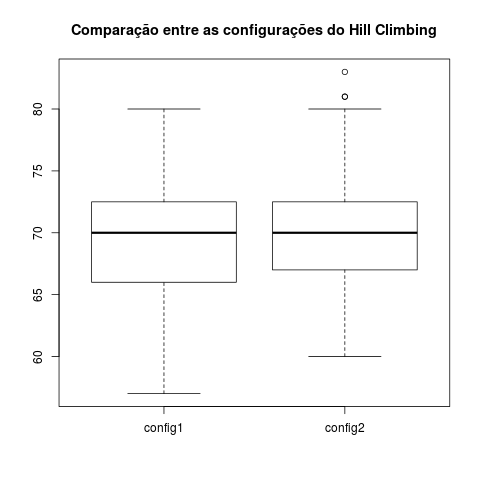
\includegraphics[width=0.6\linewidth]{img/hill-sol-queen1313col.png}
            \caption[Resultados para o benchmark queen1313col.txt]{Resultados para o benchmark \textit{queen1313col.txt}}
			\end{figure}

		\end{frame}
        
        \begin{frame}{Resultados - Hill Climbing (queen1313col - opt 13)}
        
        	\begin{table}[H]
            \centering
              \begin{tabular}{c|c}
                \textbf{config1}      & 		   \textbf{config2}                    \\ \hline \hline
               Min.   :57.00 &          Min.   :60.00          \\ \hline
               1st Qu.:66.00 &         1st Qu.:67.00           \\ \hline
               Median :70.00 &         Median :70.00           \\ \hline
               Mean   :69.47 &         Mean   :70.07           \\ \hline
               3rd Qu.:72.25 &         3rd Qu.:72.25           \\ \hline
               Max.   :80.00 &         Max.   :83.00           \\ 
              \end{tabular}
              \caption {Dados estatísticos - Hill Climbing}
        	\end{table}
        
        \end{frame}
        
        \begin{frame}{Resultados - Simulated Annealing (queen1313col - opt 13)}
        
        	\begin{figure}[H]
			\centering
            \label{fig:sol-sa-queen1313col}
            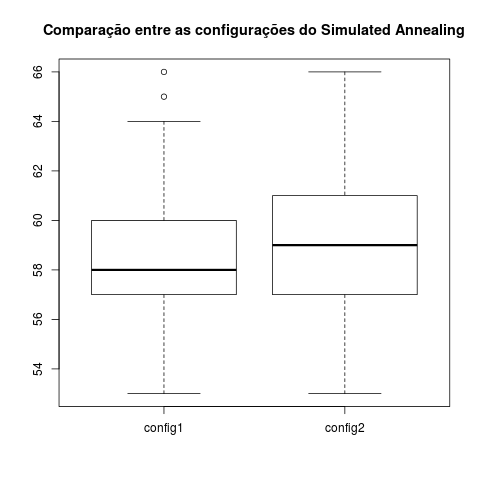
\includegraphics[width=0.5\linewidth]{img/sa-sol-queen1313col.png}
            \caption[Resultados para o benchmark queen1313col.txt]{Resultados para o benchmark \textit{queen1313col.txt}}
			\end{figure}

		\end{frame}
        
        \begin{frame}{Resultados - Simulated Annealing (queen1313col - opt 13)}
        
        	\begin{table}[H]
            \centering
              \begin{tabular}{c|c}
               \textbf{config1}       &  \textbf{config2}                        \\ \hline \hline
               Min.   :53.00 &         Min.   :53.00           \\ \hline
               1st Qu.:57.00 &          1st Qu.:57.00          \\ \hline
               Median :58.00 &         Median :59.00           \\ \hline
               Mean   :58.55 &          Mean   :59.09          \\ \hline
               3rd Qu.:60.00 &          3rd Qu.:61.00          \\ \hline
               Max.   :66.00 &          Max.   :66.00          \\
              \end{tabular}
              \caption {Dados estatísticos - Simulated Annealing}
        	\end{table}
		\end{frame}
        
        \begin{frame}{Resultados - Algoritmo Genético (queen1313col - opt 13)}
        
        	\begin{figure}[H]
			\centering
            \label{fig:sol-ga-queen1313col}
            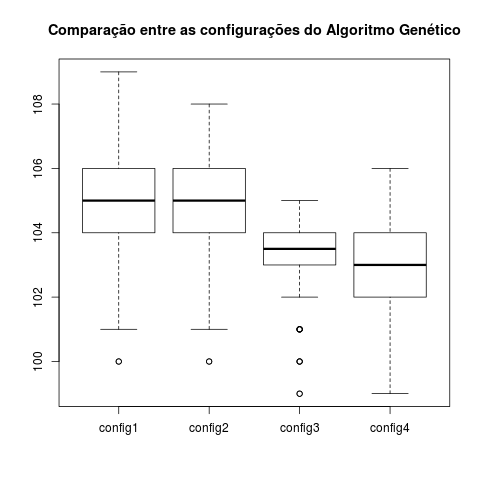
\includegraphics[width=0.5\linewidth]{img/ga-sol-queen1313col.png}
            \caption[Resultados para o benchmark queen1313col.txt]{Resultados para o benchmark \textit{queen1313col.txt}}
			\end{figure}

		\end{frame}
        
        \begin{frame}{Resultados - Algoritmo Genético (queen1313col - opt 13)}
        
        	\begin{table}[H]
            \centering
              \begin{tabular}{c|c|c|c}
               \textbf{config1}       &  \textbf{config2}              & \textbf{config3}                 & \textbf{config4}                          \\ \hline \hline
               Min.   :100.0 &         Min.   :100.0 &           Min.   : 99.0 &           Min.   : 99            \\ \hline
               1st Qu.:104.0 &         1st Qu.:104.0 &          1st Qu.:103.0  &          1st Qu.:102             \\ \hline
               Median :105.0 &         Median :105.0 &          Median :103.5  &          Median :103             \\ \hline
               Mean   :104.9 &         Mean   :104.9 &          Mean   :103.2  &           Mean   :103            \\ \hline
               3rd Qu.:106.0 &         3rd Qu.:106.0 &          3rd Qu.:104.0  &          3rd Qu.:104             \\ \hline
               Max.   :109.0 &         Max.   :108.0 &          Max.   :105.0  &          Max.   :106             \\ 
              \end{tabular}
              \caption {Dados estatísticos - Algoritmo Genético}
        	\end{table}

		\end{frame}
        
        
        
	\begin{frame}{}
		\centering
		\Huge \color{blue} \textbf{Tempo de Execução}
	\end{frame}
        
        
        
        \subsection{Resultados - Tempo de execução}
    
    	\subsubsection{mulsoli5col}
		
        \begin{frame}{Resultados - Hill Climbing (tempo-ms)}
        
        	\begin{figure}[H]
			\centering
            \label{fig:tmp-hc-mulsoli5col}
            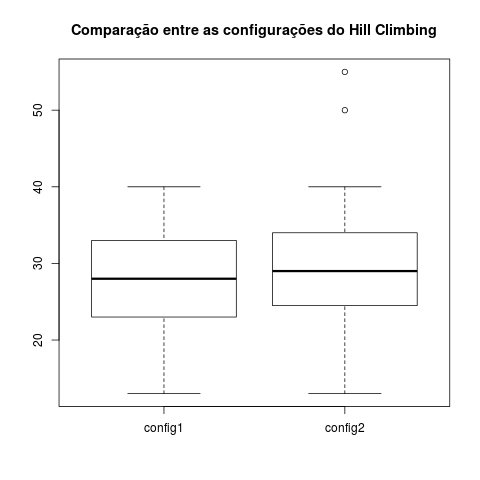
\includegraphics[width=0.6\linewidth]{img/hill-tmp-mulsoli5col.png}
            \caption[Resultados para o benchmark mulsoli5col.txt]{Resultados para o benchmark \textit{mulsoli5col.txt}}
			\end{figure}

		\end{frame}
        
        
        \begin{frame}{Resultados - Simulated Annealing (tempo-ms)}
        
        	\begin{figure}[H]
			\centering
            \label{fig:tmp-sa-mulsoli5col}
            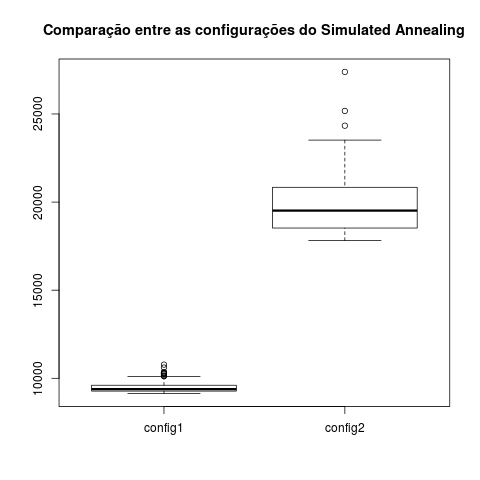
\includegraphics[width=0.6\linewidth]{img/sa-tmp-mulsoli5col.png}
            \caption[Resultados para o benchmark mulsoli5col.txt]{Resultados para o benchmark \textit{mulsoli5col.txt}}
			\end{figure}

		\end{frame}
        
        \begin{frame}{Resultados - Algoritmo Genético (tempo-ms)}
        
        	\begin{figure}[H]
			\centering
            \label{fig:tmp-ga-mulsoli5col}
            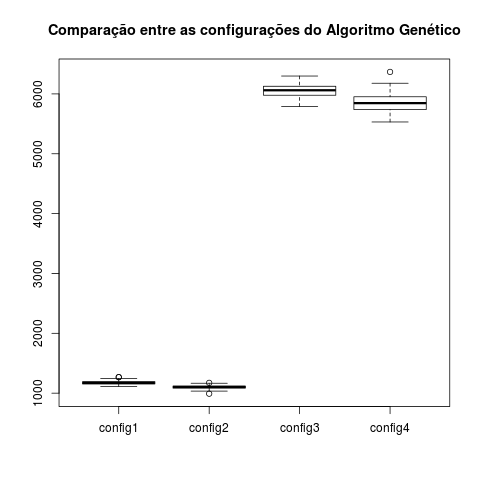
\includegraphics[width=0.6\linewidth]{img/ga-tmp-mulsoli5col.png}
            \caption[Resultados para o benchmark mulsoli5col.txt]{Resultados para o benchmark \textit{mulsoli5col.txt}}
			\end{figure}

		\end{frame}
        
        \subsubsection{queen1111col}
		
        \begin{frame}{Resultados - Hill Climbing (tempo-ms)}
        
        	\begin{figure}[H]
			\centering
            \label{fig:tmp-hc-queen1111col}
            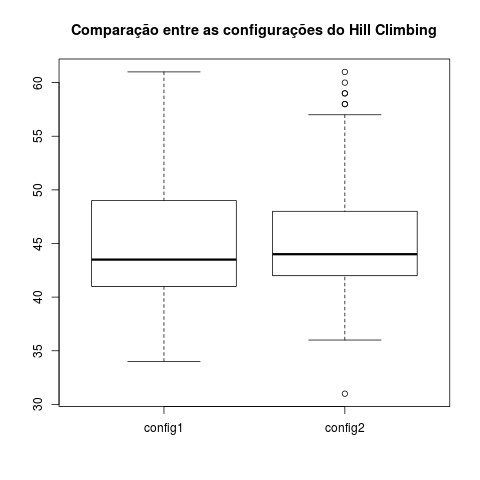
\includegraphics[width=0.6\linewidth]{img/hill-tmp-queen1111col.png}
            \caption[Resultados para o benchmark queen1111col.txt]{Resultados para o benchmark \textit{queen1111col.txt}}
			\end{figure}

		\end{frame}
        
        \begin{frame}{Resultados - Simulated Annealing (tempo-ms)}
        
        	\begin{figure}[H]
			\centering
            \label{fig:tmp-sa-queen1111col}
            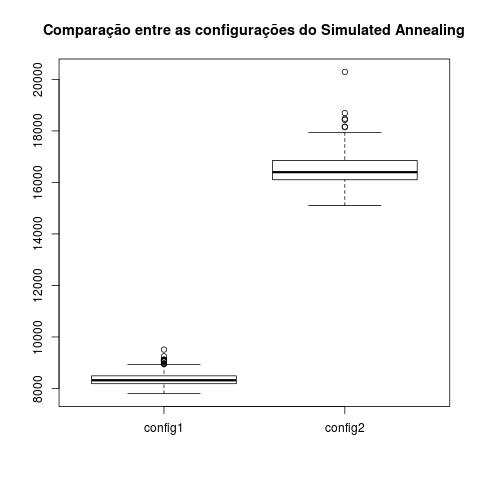
\includegraphics[width=0.6\linewidth]{img/sa-tmp-queen1111col.png}
            \caption[Resultados para o benchmark queen1111col.txt]{Resultados para o benchmark \textit{queen1111col.txt}}
			\end{figure}

		\end{frame}
        
        \begin{frame}{Resultados - Algoritmo Genético (tempo-ms)}
        
        	\begin{figure}[H]
			\centering
            \label{fig:tmp-ga-queen1111col}
            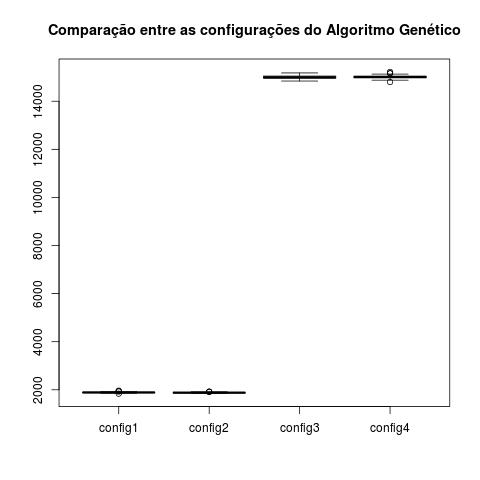
\includegraphics[width=0.6\linewidth]{img/ga-tmp-queen1111col.png}
            \caption[Resultados para o benchmark queen1111col.txt]{Resultados para o benchmark \textit{queen1111col.txt}}
			\end{figure}

		\end{frame}
        
        \subsubsection{queen1313col}
		
        \begin{frame}{Resultados - Hill Climbing (tempo-ms)}
        
        	\begin{figure}[H]
			\centering
            \label{fig:tmp-hc-queen1313col}
            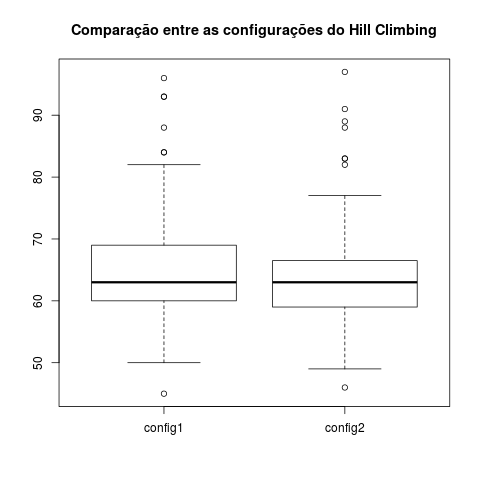
\includegraphics[width=0.6\linewidth]{img/hill-tmp-queen1313col.png}
            \caption[Resultados para o benchmark queen1313col.txt]{Resultados para o benchmark \textit{queen1313col.txt}}
			\end{figure}

		\end{frame}
        
        \begin{frame}{Resultados - Simulated Annealing (tempo-ms)}
        
        	\begin{figure}[H]
			\centering
            \label{fig:tmp-sa-queen1313col}
            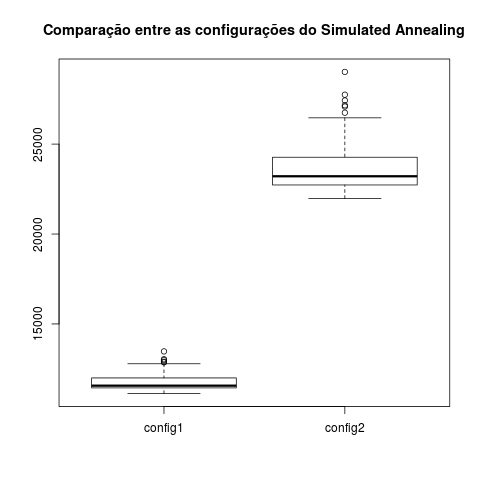
\includegraphics[width=0.6\linewidth]{img/sa-tmp-queen1313col.png}
            \caption[Resultados para o benchmark queen1313col.txt]{Resultados para o benchmark \textit{queen1313col.txt}}
			\end{figure}

		\end{frame}
        
        \begin{frame}{Resultados - Algoritmo Genético (tempo-ms)}
        
        	\begin{figure}[H]
			\centering
            \label{fig:tmp-ga-queen1313col}
            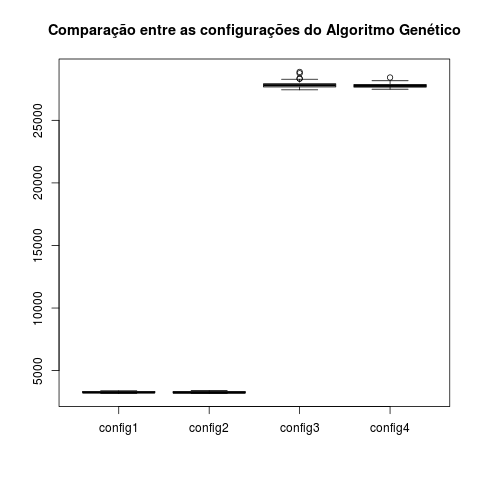
\includegraphics[width=0.6\linewidth]{img/ga-tmp-queen1313col.png}
            \caption[Resultados para o benchmark queen1313col.txt]{Resultados para o benchmark \textit{queen1313col.txt}}
			\end{figure}

		\end{frame}
	
    
    
\section{Conclusão}
	\begin{frame}{}
		\centering
		\Huge \color{blue} \textbf{Conclusão}
	\end{frame}
    
	\begin{frame}{Conclusão - Algoritmos}
		
		\begin{itemize}
			
			\item Ambos, Simulated Annealing e Hill Climbing, apresentaram boas soluções, com destaque para o SA;
			
			\bigskip
			\item Já a implementação do Algoritmo Genético precisa de mais atenção.
           	
            \begin{itemize}
				\item Desenvolver métodos de mutação mais eficazes assim como a seleção de pais e outros;
                
                \bigskip
                
                \item Realizar uma mudança para que \textit{todo} indivíduo gerado seja \textit{válido}.
			\end{itemize}
            
			\bigskip
            \bigskip
			
			\item Para obter uma melhora significativa nos resultados dos algoritmos, deve-se:
            \begin{itemize}
                \item Realizar uma pesquisa aprofundada do estado da arte;
                
               \bigskip
               
            	\item Investir em um método de perturbação mais eficiente;
			\bigskip
                \item Variar mais os parâmetros e utilizar mais benchmarks.
                
            \end{itemize}
			
		\end{itemize}
		
	\end{frame}
    
	
	\begin{frame}{Conclusão - Trabalho Desenvolvido}
		
		\begin{itemize}
			
			\item O Simulated Annealing se mostrou com melhor resultados
            
            \bigskip
            
            \item Porém, isso não serve para inferir que o Algoritmo Genético ou Hill Climbing são ruins, pois, para afirmar isso, depende de:
            
            
            \begin{itemize}
				\item Implementações específicas;
                \bigskip
                \item Próprio problema em si (Representação, essência...);
                \bigskip
                \item Variação de parâmetros e uma análise experimental mais robusta.
			\end{itemize}
            
			
		\end{itemize}
		
	\end{frame}

\logo{\pgfputat{\pgfxy(-1.6,-0.1)}{\pgfbox[center,base]{
\includegraphics[width=3cm]{img/logo.jpg}}}}

\frame{\titlepage}

\setbeamertemplate{logo}{}


	
\begin{thebibliography}{99}
		
	\bibitem{Diego}SILVA, Diego Mello da. \textbf{Métodos Heurísticos}: Fundamentos. 2014. Disponível em: $<$\url{http://goo.gl/GxjNUK}$>$. Acesso em: 05 fev. 2015.
    
    \bibitem{kempe1879}KEMPE, A. B. On the Geographical Problem of the Four Colours. \textbf{American Journal of Mathematics}, [S.I.], 1879. n. 2, p. 193-200.
    
    \bibitem{Lopes2013}LOPES, H. S., RODRIGUES, L. C. A., STEINER, M. T. A. \textbf{Meta-heurísticas em Pesquisa Operacional}. Ominipax, 2013.
	
	\bibitem{Ziviani}ZIVIANI, Nivio. \textbf{Projeto de Algoritmos: Introdução}. 2010. Disponível em: $<$\url{http://www2.dcc.ufmg.br/livros/algoritmos/cap1/slides/pascal/completo1/cap1.pdf}$>$. Acesso em: 05 fev. 2015.
	
\end{thebibliography}


\end{document}